\documentclass[a4paper,twoside,titlepage,openright]{book}
\usepackage[MeX]{polski}
\usepackage[utf8]{inputenc}
\usepackage{enumitem} % słownik pojęć
\usepackage{amsmath}
\usepackage{tabularx} % tabele
\usepackage[usenames,dvipsnames,svgnames,table]{xcolor} % kolory jak~się chce gdzieś użyć
\usepackage{graphicx} % żeby ryciny i~zdjęcia były
\usepackage{listings} % syntax highlighting
\usepackage{verbatimbox} % marginesy dla~tabel
\usepackage{emptypage} % usuwa nagłówki i~numery stron z~pustych stron
\usepackage{afterpage} % to zapobiega ustawianiu obrazka PO tym

% PAGE LAYOUT
%\usepackage{showframe} % debug
\marginparwidth 0pt
\marginparsep 0pt
\usepackage[top=3.5cm,bottom=3.5cm,inner=3.5cm,outer=2.5cm]{geometry}

% HEADER, FOOTER
\usepackage{fancyhdr} 
\pagestyle{fancy}

%kropki w~spisie tresci
\makeatletter
\def\numberline#1{\hb@xt@\@tempdima{#1.\hfil}}
\makeatother

% CHAPTER TITLE

%kropki po~tytułach rodziałów
\makeatletter
\def\@makechapterhead#1{%
  \vspace*{50\p@}%
  {\parindent \z@ \raggedright \normalfont
	\ifnum \c@secnumdepth >\m@ne
	  \if@mainmatter
	   \huge\bfseries \@chapapp\space \thechapter.
	   \par\nobreak
	   \vskip 20\p@
	\fi
   \fi
   \interlinepenalty\@M
   \Huge \bfseries #1\par\nobreak
   \vskip 40\p@
  }}
\makeatother

% SPIS TREŚCI

%kropki w~spisie tresci
\makeatletter
\def\numberline#1{\hb@xt@\@tempdima{#1.\hfil}}
\makeatother

% TYTUŁY ROZDZIAŁÓW

%kropki po~tytułach rozdziałów
\makeatletter
\renewcommand*\@seccntformat[1]%
{\csname the#1\endcsname.\enspace}
\makeatother


% KONFIGURACJA WYGLĄDU NAGŁÓWKA TEGO CO SIĘ POWTARZA

\fancyhead{} 
\fancyhead[LE]{\rightmark}
\fancyhead[RO]{\leftmark}

% WYGLĄD TABEL

% vertical padding
\renewcommand{\arraystretch}{1.5}

% CODE LISTINGS 

\definecolor{mygreen}{rgb}{0,0.6,0}
\definecolor{mygray}{rgb}{0.5,0.5,0.5}
\definecolor{mymauve}{rgb}{0.58,0,0.82}

\lstset{ %
%frame=lines,
aboveskip=1.5em,
    belowcaptionskip=1.5em,
    xleftmargin=0.5cm,
  backgroundcolor=\color{white},   % choose the background color
  %basicstyle=\footnotesize,        % size of fonts used for the code
  breaklines=true,                 % automatic line breaking only at whitespace
  captionpos=b,                    % sets the caption-position to bottom
  commentstyle=\color{mygreen},    % comment style
  escapeinside={\%*}{*)},          % if you want to add LaTeX within your code
  keywordstyle=\color{blue},       % keyword style
  stringstyle=\color{mymauve},     % string literal style
}

\definecolor{maroon}{rgb}{0.5,0,0}
\definecolor{darkgreen}{rgb}{0,0.5,0}

\lstdefinelanguage{XML}
{
  basicstyle=\ttfamily,
  morestring=[s]{"}{"},
  morecomment=[s]{?}{?},
  morecomment=[s]{!--}{--},
  commentstyle=\color{darkgreen},
  moredelim=[s][\color{black}]{>}{<},
  moredelim=[s][\color{red}]{\ }{=},
  stringstyle=\color{blue},
  identifierstyle=\color{maroon},
  morekeywords={Page.DataContext,viewModel:NameViewModel}
}

%\setmonofont{Consolas} %to be used with XeLaTeX or LuaLaTeX
\definecolor{bluekeywords}{rgb}{0,0,1}
\definecolor{greencomments}{rgb}{0,0.5,0}
\definecolor{redstrings}{rgb}{0.64,0.08,0.08}
\definecolor{xmlcomments}{rgb}{0.5,0.5,0.5}
\definecolor{types}{rgb}{0.17,0.57,0.68}

%Poprawne wyświetlanie listingów c#
\lstset{language=[Sharp]C,
%captionpos=b,
%numbers=left, %Nummerierung
%numberstyle=\tiny, % kleine Zeilennummern
%frame=lines, % Oberhalb und unterhalb des Listings ist eine Linie
showspaces=false,
showtabs=false,
breaklines=true,
showstringspaces=false,
breakatwhitespace=true,
escapeinside={(*@}{@*)},
commentstyle=\color{greencomments},
morekeywords={partial, var, value, get, set},
keywordstyle=\color{bluekeywords},
stringstyle=\color{redstrings},
basicstyle=\ttfamily\small,
}




\begin{document}

% ################################
%        STRONA TYTUŁOWA
% ################################

\begin{titlepage}

%\newgeometry{inner=3cm,outer=3cm}

\vspace*{1cm}
\begin{center}
\begin{Large}
Uniwersytet Mikołaja Kopernika\\[1mm]
Wydział Matematyki i~Informatyki\\[1mm]
\end{Large}
\end{center}

\vfill

\begin{center}
{\Large Paweł Marcin Chojnacki}\\
nr albumu: 260082\\
informatyka
\end{center}

\vfill

\begin{center}
{\Large Praca magisterska}
\end{center}

\vspace{0.5cm}

\begin{center}
{\Huge \textbf{Porównanie wydajności współczesnych architektur sieci neuronowych}}
\end{center}

\vspace{2cm}
\hfill
\begin{minipage}{6.5cm}
Opiekun pracy dyplomowej\\
dr hab. Piotr Wiśniewski
\end{minipage}

\vfill

\begin{center}
Toruń 2018
\end{center}

\end{titlepage}

% odwracamy kartkę ze~stroną tytułową to nic nie~ma z~drugiej strony -> pusta strona
\clearpage{\pagestyle{empty}\cleardoublepage}

\tableofcontents

% ################################
%        SŁOWNIK POJĘĆ
% ################################

\chapter*{Słownik pojęć}
\markboth{}{Słownik pojęć}
\addcontentsline{toc}{chapter}{Słownik pojęć}
\begin{description}[style=nextline]
	\item[Klasyfikacja binarna] Klasyfikacja binarna polega na jak najdokładniejszym stwierdzeniu posiadania cechy lub przynależności do kategorii danego obiektu.
Najczęściej używane metody do klasyfikacji binarnej to: drzewa decyzyjne 
Dane wejściowe należy przedstawić w formie macierzy. Każdy przykład do treningu i później klasyfikacji, musi być tych samych wymiarów. Wyjściem algorytmu klasyfikacji binarnej jest wektor z prawdopodobieństwem klasyfikacji każdego z przykładów. Wizualizacja funkcji, klasyfikującej czerwone i zielone kółka.
W klasyfikacji binarnej przykłady zapisuje się jako pary (x,y) - x to wartość danego przykładu, y to odpowiedź na pytanie czy przykład posiada klasyfikowaną cechę.
Mając m przykładów: {(x1,y1),(x2,y2),(x3,y3),...,(xm,ym)}. Dla uproszczenia obliczeń, zwyczajowo stosuje się zapis macierzowy:
[ x(1), x(2),..., x(n) ]
[ x(1), x(2),..., x(n) ]
[ x(1), x(2),..., x(n) ]
[ x(1), x(2),..., x(n) ]
Jedna kolumna to jeden przykład, dlatego szerokość macierzy to m.
Zbiór cech przykładów można również uprościć i zapisać je w formie wektora Y = [y1,y2,...ym]
	\item[Regresja logistyczna] Metoda statystyczna używana do analizy zbioru danych, w którym mam więcej niż jedną zmienną determinującą wyjście. Wyjściem jest prawdopodobieństwo wystąpienia klasyfikowanego elementu. Algorytm regresji logistycznej przyjmuje na wejściu dane: n-wymiarowy wektor liczb rzeczywistych [np. Obraz], zestaw wag o tych samych wymiarach, liczba rzeczywista, bias.
Do wygenerowania wyjścia, wystarczy obliczyć y = wT (wagi transponowane) * x (wejście) + b (bias). Należy jeszcze zastosować operację, która pozwoli na ustawienie parametrów w przedziale 0-1. Całe powyższe równanie użyć jako wejście do funkcji sigmoidy. Sigm(z) = 1 / 1 + e-z. Jeśli z jest duże, sigmoida będzie bliska 1, jeśli z jest liczbą ujemną, sigmoida zbliży się do 0.
	\item[Funkcja kosztu] Funkcja do trenowania modelu regresji logistycznej. Mając zestawy treningowe, można wytrenować algorytm tak, aby podawał wartości prawdopodobieństwa jak najbliższe zestawu treningowego. Chcemy ustawić wagi i bias tak, aby te parametry dawały prawidłową odpowiedź dla każdego przykładu uczącego. Funkcja kosztu ma następujący wzór:
	\item[Metoda gradientu prostego] Algorytm pozwalający znaleźć minimum funkcji. Wyobrażając sobie płaszczyznę funkcji dla wszystkich możliwych argumentów, algorytm przechodzi z losowo rozpoczętego miejsca w miejsce gdzie jest najgłębiej. Mając funkcję kosztu J(w,b) szukamy miejsca w którym błąd algorytmu jest jak najmniejszy.
	\item[Wykres obliczeniowy] (ang. Computation graph). Dekompozycja wyrażenia w pojedyncze atomowe kroki. Używany do optymalizowania funkcji. Przydaje się podczas ręcznej analizy funkcji błędu.
	\item[Funkcje aktywacji] - funkcja definiująca 
	\item[Pooling] - technika polegająca na zmniejszeniu danych wejściowych. Aby zmniejszyć obraz ustala się rozmiar filtra oraz wielkość kroku. Następuje przejscie po całym obrazie (po nałożeniu filtra) i wybiera się max z całego obszaru filtra do nowej macierzy. Pozwala to ograniczyć ilość parametrów i wyodrębnić konkretne cechy obiektu.
	\item[Konwolucja]
	\item[Wsteczna propagacja błędu] 
	\item[Dropout]
	\item[ReLU]
	\item[Softmax]
	\item[Epoka ang. Epoch]
	\item[Model]
\end{description}
 
% ################################
%        WSTĘP
% ################################

\chapter*{Wstęp}
\markboth{}{Wstęp}
\addcontentsline{toc}{chapter}{Wstęp}


\clearpage{\pagestyle{empty}\cleardoublepage}
\chapter{Neurony}

\section{Co to jest sieć neuronowa?}

\section{Jak uczyć sieć zachowań?}
\subsection*{Uczenie nadzorowane}
\subsection*{Uczenie nienadzorowane}

\section{Elementy sieci neuronowych}
\subsection{Metoda gradientu prostego}
\subsection{Funkcje aktywacji}
\subsection{Wykres obliczeniowy}
\subsection{Propagacja i wsteczna propagacja błędu}
\subsection{Parametry}
\subsection{Hiperparametry}
\subsection{Jak zbudować sieć neuronową}

\chapter{Deep Learning}

\section{Techniki w deep learning}

\subsection{Sieci neuronowe}
\subsection{Convolutional Neural Networks}
\subsection{Recurrent Neural Networks}
\subsection{Fully Convolutional Networks}

\section{Przegląd bibliotek}
\subsection{Tensorflow}
\subsection{Keras}
\subsection{PyTorch}
\subsection{deeplearning.js}
\subsection{Paddle}
\subsection{MXNet}
\subsection{Caffe2}

\chapter{Architektura}
\section{Poglądy profesora Tadeusiewicza}
\subsection{CNTK}
Sieci neuronowe można ułożyć na nieskończenie wiele sposobów. Aby uzyskać dobre rezultaty należy sprawdzić kilka architektur i jak się zachowują dla dla posiadanych zbiorów danych i zadanych hiperparametrów.
W zależności od typu architektury sieci można osiągnąć zupełnie inne wyniki uczenia dla tych samych algorytmów. 
Architektury różnią się właściwie wszystkim, ilością warstw ukrytych ilością neuronów w warstwie ukrytej. 
Poglądy Tadeusiewicza na architekturę sieci neuronowych.

“Właśnie taka (warstwowa) struktura sieci wyjątkowo łatwo i wygodnie da się wytwarzać zarówno w formie modelu elektronicznego, jak i da się symulować w formie programu komputerowego. Dlatego badacze przyjęli właśnie strukturę warstwową i od tej pory stosują ją we wszystkich sztucznych sieciach neuronowych. Z pełną wiernością biologicznemu oryginałowi ma to niewiele wspólnego, ale jest praktyczne i wygodne. W związku z tym wszyscy tak postępują, nie martwiąc się ani przesłankami biologicznymi, ani dowodami wskazującymi, że architektura sieci bardziej wymyślnie dostosowanej do charakteru zadania może znacznie lepiej realizować stawiane zadania.”

Tak napisał w 2007 roku, kiedy architektury sieci nie miały miały większego znaczenia ponieważ większość sieci była stosunkowo płytka (do 5 warstw ukrytych). Zbiory na których pracowano były stosunkowo niewielkie w porównaniu z dzisiejszymi zasobami skatalogowanych obrazów. 
Obecnie istnieją dowody (choćby coroczne zawody ImageNet, w których udowadnia się że struktura sieci ma znaczenie. Może poprawić szybkość i dokładność uczenia). Profesor jest ekspertem w dziedzinie sieci neuronowych, jednak jego książki i poglądy są z lat 1990 - 2010. Późniejsze jego prace są dużo mniej znane.

\section{Przegląd sprawdzonych architektur}
\subsection{AlexNet}
 [Alex Krizhevsky, Ilya Sutskever, Geoffrey E. Hinton, 2012] - konwolucyjna sieć neuronowa napisana przy użyciu CUDA pod zawody ImageNet. Została wytrenowana do sklasyfikowania 1,2 miliona obrazów podzielonych na 1000 klas. W testach top-1 i top-5 uzyskała wartości kolejno 37,5\% i 17\%, co jest wynikiem niesamowicie wysokim na 2012 rok. Sieć neuronowa zawiera 60 milionów parametrów i 650 000 neuronów.
Architekturę tworzy 8 warstw, gdzie pierwsze 5 to warstwy konwolucyjne, a pozostałe 3 są warstwami w pełni połączonymi, ta ostatnia ma oczywiście 1000 wyjść z funkcji softmax.
AlexNet znacząco przewyższyła swoją wydajnością poprzednich uczestników i wygrała zawody redukując błąd top-5 do 15,32\%. Drugie miejsce to błąd ok 26.2\% (nie była to CNN).
Sieć jest głęboką modyfikacją architektury Yann’a LeCunn’a. AlexNet była zaplanowana na dwie karty graficzne, stąd rozdzielenie przepływu informacji na 2 części. Trenowanie sieci na 2 GPU było nowością na te czasy. Sieć została wytrenowana na zbiorze ImageNet. Do wyliczenia funkcji nieliniowych były używane ReLU (tutaj po raz pierwszy okazało się że ReLU działa dużo szybciej niż tanh). Sieć o której będą uczyły się dzieci na lekcjach historii.

\begin{figure}[h]
	\centering
			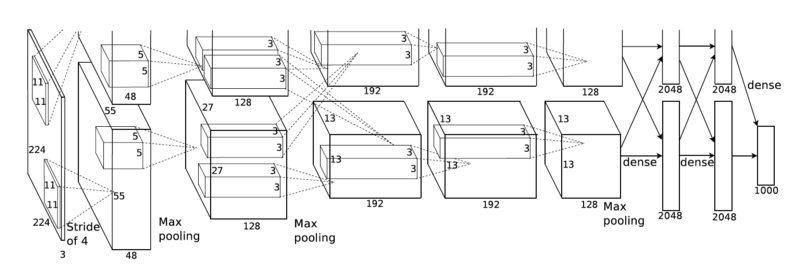
\includegraphics[resolution=120]{AlexNet.png}
		\caption{Architektura sieci AlexNet}
\end{figure}

\subsection{LeNet}
Jest to obecnie mało znacząca architektura. Pierwsze praktyczne zastosowanie sieci konwolucyjnych jeszcze w latach 90’tych. Używana była do prostych zadań: czytanie kodów pocztowych, liczb.

\begin{figure}[h]
	\centering
			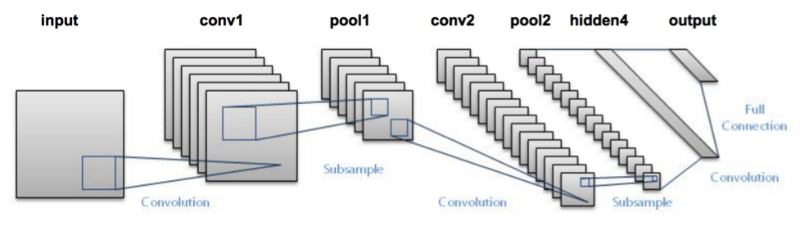
\includegraphics[resolution=120]{LeNet.png}
		\caption{Architektura sieci LeNet}
\end{figure}

\subsection{VGG Net}
 [Simoyan i Zisserman, 2014] - sieć złożona z 16 warstw konwolucyjnych, która charakteryzuje się małymi filtrami i duża głębokość sieci.
W trakcie trenowania sieci wyjście jest ustawione na ustalony rozmiar (224 x 224 x 3). Przetwarzanie wstępne obejmuje odjęcie mediany wartości RGB dla każdego piksela. Zdjęcie jest przetwarzanie przez stos warstw konwolucyjnych, gdzie używane są filtry o bardzo małym polu widzenia (3x3) [najmniejszy możliwy rozmiar by móc rozpoznać kierunek]. Operacja Max-pooling jest wykonana na polu 4 pikseli, co pokazuje że jest to pobieranie jak najmniejszych cech z obrazu. Ukryte warstwy są wyposażone w nieliniową funkcję aktywacji ReLU. Po stosie warstw konwolucyjnych, następuje nałożenie 3 warstw w pełni połączonych (to takie duże warstwy zawierające wszystkie cechy?). Pierwsze dwie mają 4096 kanałów, trzecia już tylko 1000 (po jednym kanale na klasę obiektu). Obecnie architektura ta jest dość popularnym wyborem dla wyodrębniania cech ze zdjęć. Konfiguracje wag dla zbioru obrazów z ImageNet są dostępne online. W tej sieci problemem jest 140 milionów parametrów, którymi czasem trzeba zarządzać.

\subsection{GoogleNet / Inception}
[Christian Szegedy, Wei Liu, Yangqing Jia, Pierre Sermanet, Scott Reed, Dragomir Anguelov, Dumitru Erhan, Vincent Vanhoucke, Andrew Rabinovich, 2014] - produkt jak nazwa wskazuje wyszedł z firmy Google. Charakteryzuje się przełomową poprawą użycia zasobów wewnętrznych. ImageNet jest zaprojektowana na jak największą szerokość i głębokość jednocześnie utrzymując stałe zużycie mocy obliczeniowej. Optymalizacja jakości opiera się na zasadzie Hebbian’a (jest to teoria neuronauki, która mówi o adaptacji neuronów w trakcie nauki). Błędy klasyfikacji wynoszą top-1: 17,2\% i top-5: 3,58\% (dla v3). Sieć składa się łącznie z 22 warstw. Sieć jest modułowa, gdzie każdy moduł pełni rolę wielopoziomowego ekstraktora cech przeliczającego konwolucje na macierzach rozmiarów 1x1, 3x3, 5x5. Zaletą tej architektury są bardzo małe rozmiary wag (mniej niż 100MB dla v3). Kolejną ważną zaletą jest ilość parametrów, tylko 4 miliony co jest wynikiem 12 razy lepszym od AlexNet. Jest to jedna z najbardziej złożonych sieci względem architektury modułowej. W wersji naiwnej każda warstwa posiada 4 ekstraktory cech (3 konwolucyjne i jedną 3x3 max pooling), następnie wartości te są składane i wysyłane do warstwy wyżej. Do poprawienia wydajności obliczeniowej pozbyto się warstwy “w pełni połączonej”.

\subsection{ResNet}
[Kaiming He et al, 2015]  - architektura oparta na mikro modułach. Charakteryzuje się możliwością odrzucania połączeń i posiada ogromny moduł na normalizację zbioru iteracji (batch normalization). Normalizacja jest pomysłem zaczerpniętym z rekurencyjnych sieci neuronowych. Ta technika pozwala stworzyć sieć ze 152 warstwami ukrytymi przy zachowaniu złożoności mniejszej niż VGG.

\begin{figure}[h]
	\centering
			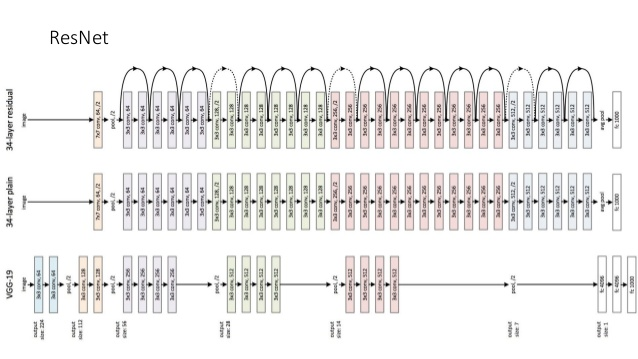
\includegraphics[resolution=120]{ResNet.png}
		\caption{Architektura sieci ResNet}
\end{figure}

\subsection{ResNeXt}
[Saining Xie, Ross Girshick, Piotr Dolla ́r Zhuowen Tu Kaiming He, 2017] - modularyzowalna 

\begin{figure}[h]
	\centering
			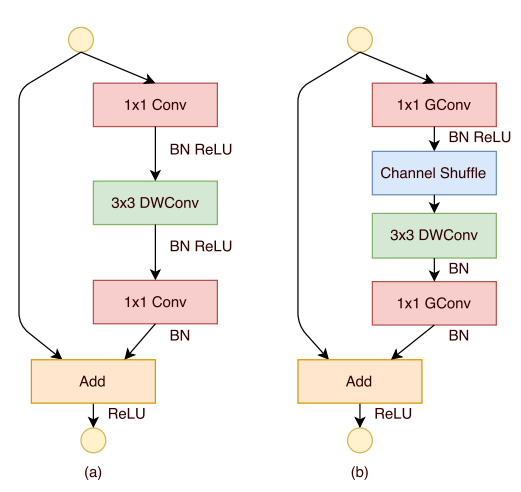
\includegraphics[resolution=120]{ResNeXt.png}
		\caption{Architektura sieci ResNeXt}
\end{figure}

\subsection{RCNN}
\begin{figure}[h]
	\centering
			\includegraphics[resolution=120]{RCNN.png}
		\caption{Architektura sieci RCNN}
\end{figure}

\subsection{YOLO - You Only Look Once }
[Joseph Redmon, Santosh Divvala, Ross Girshick, Ali Farhadi, 2016] - You Only Look Once jest systemem wykrywania obiektów w czasie rzeczywistym. Obraz jest dzielony na części oddzielonymi od sieibie prostokątami, ..???
Cały przepływ danych do wykrycia obiektów jest jedną siecią, dlatego może być zoptymalizowany 
\begin{figure}[h]
	\centering
			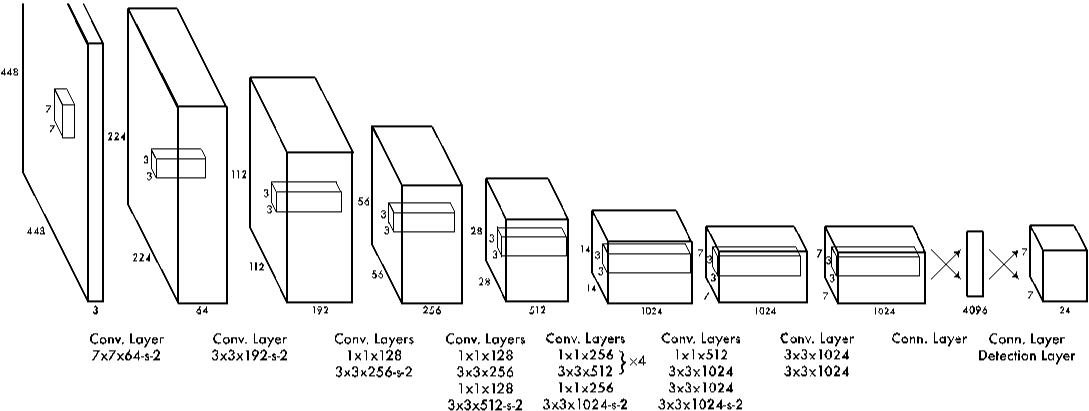
\includegraphics[resolution=120]{YOLO.png}
		\caption{Architektura sieci YOLO}
\end{figure}

\subsection{SqueezeNet}

\begin{figure}[h]
	\centering
			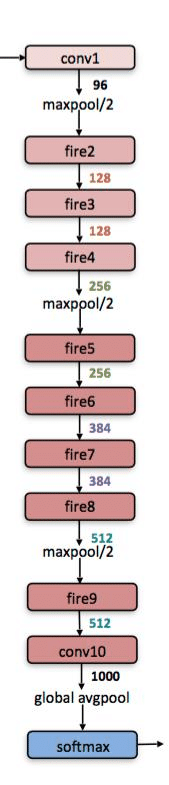
\includegraphics[resolution=120]{SqueezeNet.png}
		\caption{Architektura sieci SqueezeNet}
\end{figure}

\subsection{SegNet}
\begin{figure}[h]
	\centering
			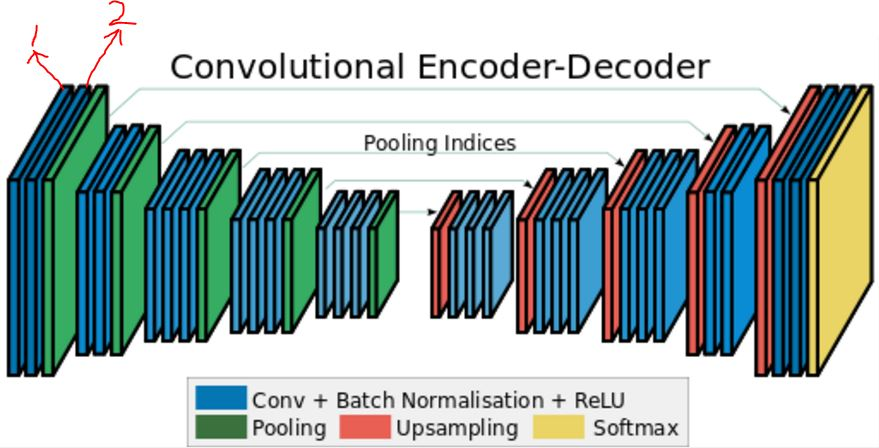
\includegraphics[resolution=120]{SegNet.png}
		\caption{Architektura sieci SegNet}
\end{figure}

\subsection{Generative Adversarial Network}
[Ian J. Goodfellow, Jean Pouget-Abadie, Mehdi Mirza, Bing Xu, David Warde-Farley, Sherjil Ozair†, Aaron Courville, Yoshua Bengio‡, 2014] - w skrócie GAN. Są architekturą sieci neuronowych skomponowanych z dwóch sieci przeciwstawionych wobec siebie. Zaprojektowane na uniwersytecie w Montrealu (gdzie powstało większość przełomów dotyczących neuronów) przez największe obecnie autorytety w dziedzinie. GAN obudził duze nadzieje na szybkie i "twórcze" działania algorytmów, jego najczęstszym zastosowaniem jest tworzenie komputerowych "dzieł sztuki". Jak to działa? Jedna sieć generuje kandydatów, a druga ich ocenia wytworzone obiekty. W ten sposób obie sieci uczą się od siebie wzajemnie. 

\begin{figure}[h]
	\centering
			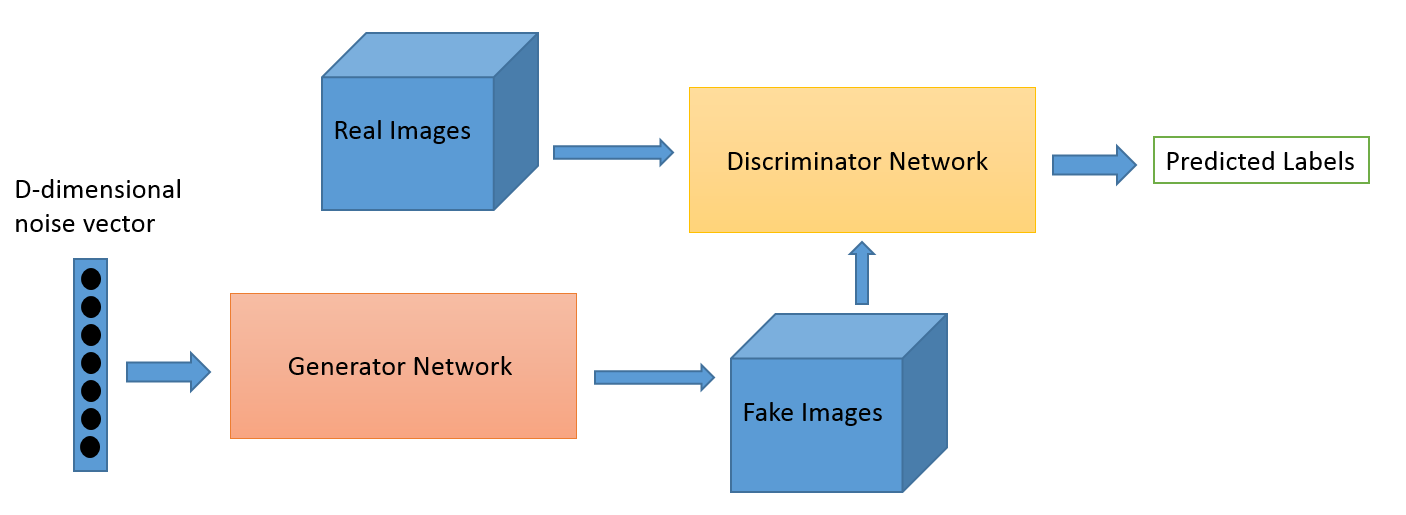
\includegraphics[resolution=120]{GAN.png}
		\caption{Architektura sieci GAN}
\end{figure}

% ################################
%        PODSUMOWANIE
% ################################

\chapter{Podsumowanie} 

\addcontentsline{toc}{chapter}{Spis rysunków}
\listoffigures

% ################################
%        BIBLIOGRAFIA
% ################################

\addcontentsline{toc}{chapter}{Bibliografia}
\begin{thebibliography}{99}

\bibitem{deeplearningbook} \textsc{Goodfellow I., Bengio Y, Courville A.:}
\textit{Deep Learning (Adaptive Computation and Machine Learning series)}, The MIT Press, 2016, ISBN 978-0262035613.

\bibitem{medicalImage} \textit{Medical Image Retrieval using Deep Convolutional Neural Network}, 
\texttt{https://arxiv.org/pdf/1703.08472.pdf}, \\dostęp: 10.04.2018.

\bibitem{fastAI} \textit{Practical Deep Learning for Coders}, 
\texttt{http://course.fast.ai}, \\dostęp: 10.04.2018.

\bibitem{resnextArxiv} \textit{Aggregated Residual Transformations for Deep Neural Networks}, 
\texttt{https://arxiv.org/pdf/1611.05431.pdf}, \\dostęp: 10.04.2018.

\bibitem{alexnetNips} \textit{ImageNet Classification with Deep Convolutional Neural Networks}, 
\texttt{https://papers.nips.cc/paper/4824-imagenet-classification-with-deep-convolutional-neural-networks.pdf}, \\dostęp: 10.04.2018.

\bibitem{lecun} \textit{Gradient-Based Learning Applied to Document Recognition}, 
\texttt{http://yann.lecun.com/exdb/publis/pdf/lecun-01a.pdf}, \\dostęp: 10.04.2018.

\bibitem{ganArxiv} \textit{Generative Adversarial Nets}, 
\texttt{https://arxiv.org/pdf/1406.2661v1.pdf}, \\dostęp: 10.04.2018.

\bibitem{dropout} \textit{Dropout: A Simple Way to Prevent Neural Networks from Overfitting}, 
\texttt{https://www.cs.toronto.edu/~hinton/absps/JMLRdropout.pdf}, \\dostęp: 10.04.2018.

\bibitem{relu} \textit{Rectified Linear Units Improve Restricted Boltzmann Machines
}, 
\texttt{http://www.cs.toronto.edu/~fritz/absps/reluICML.pdf}, \\dostęp: 10.04.2018.

\bibitem{rCNN} \textit{Faster R-CNN: Towards Real-Time Object Detection with Region Proposal Networks}, 
\texttt{https://arxiv.org/pdf/1506.01497v3.pdf}, \\dostęp: 10.04.2018.

\bibitem{ZFNet} \textit{Practical Deep Learning for Coders}, 
\texttt{https://arxiv.org/pdf/1311.2901v3.pdf}, \\dostęp: 10.04.2018.

\bibitem{VGGNet} \textit{VERY DEEP CONVOLUTIONAL NETWORKS FOR LARGE-SCALE IMAGE RECOGNITION}, 
\texttt{https://arxiv.org/pdf/1409.1556v6.pdf}, \\dostęp: 10.04.2018.

\bibitem{googleNet} \textit{Going Deeper with Convolutions}, 
\texttt{https://www.cv-foundation.org/openaccess/content\_cvpr\_2015/papers/Szegedy\_Going\_Deeper\_With\_2015\_CVPR\_paper.pdf}, \\dostęp: 10.04.2018.

\bibitem{microsoftResNet} \textit{Deep Residual Learning for Image Recognition}, 
\texttt{https://arxiv.org/pdf/1512.03385v1.pdf}, \\dostęp: 10.04.2018.

\end{thebibliography}
\end{document}